\documentclass[]{article}
\usepackage{lmodern}
\usepackage{amssymb,amsmath}
\usepackage{ifxetex,ifluatex}
\usepackage{fixltx2e} % provides \textsubscript
\ifnum 0\ifxetex 1\fi\ifluatex 1\fi=0 % if pdftex
  \usepackage[T1]{fontenc}
  \usepackage[utf8]{inputenc}
\else % if luatex or xelatex
  \ifxetex
    \usepackage{mathspec}
  \else
    \usepackage{fontspec}
  \fi
  \defaultfontfeatures{Ligatures=TeX,Scale=MatchLowercase}
\fi
% use upquote if available, for straight quotes in verbatim environments
\IfFileExists{upquote.sty}{\usepackage{upquote}}{}
% use microtype if available
\IfFileExists{microtype.sty}{%
\usepackage{microtype}
\UseMicrotypeSet[protrusion]{basicmath} % disable protrusion for tt fonts
}{}
\usepackage[margin=1in]{geometry}
\usepackage{hyperref}
\hypersetup{unicode=true,
            pdfborder={0 0 0},
            breaklinks=true}
\urlstyle{same}  % don't use monospace font for urls
\usepackage{graphicx,grffile}
\makeatletter
\def\maxwidth{\ifdim\Gin@nat@width>\linewidth\linewidth\else\Gin@nat@width\fi}
\def\maxheight{\ifdim\Gin@nat@height>\textheight\textheight\else\Gin@nat@height\fi}
\makeatother
% Scale images if necessary, so that they will not overflow the page
% margins by default, and it is still possible to overwrite the defaults
% using explicit options in \includegraphics[width, height, ...]{}
\setkeys{Gin}{width=\maxwidth,height=\maxheight,keepaspectratio}
\IfFileExists{parskip.sty}{%
\usepackage{parskip}
}{% else
\setlength{\parindent}{0pt}
\setlength{\parskip}{6pt plus 2pt minus 1pt}
}
\setlength{\emergencystretch}{3em}  % prevent overfull lines
\providecommand{\tightlist}{%
  \setlength{\itemsep}{0pt}\setlength{\parskip}{0pt}}
\setcounter{secnumdepth}{0}
% Redefines (sub)paragraphs to behave more like sections
\ifx\paragraph\undefined\else
\let\oldparagraph\paragraph
\renewcommand{\paragraph}[1]{\oldparagraph{#1}\mbox{}}
\fi
\ifx\subparagraph\undefined\else
\let\oldsubparagraph\subparagraph
\renewcommand{\subparagraph}[1]{\oldsubparagraph{#1}\mbox{}}
\fi

%%% Use protect on footnotes to avoid problems with footnotes in titles
\let\rmarkdownfootnote\footnote%
\def\footnote{\protect\rmarkdownfootnote}

%%% Change title format to be more compact
\usepackage{titling}

% Create subtitle command for use in maketitle
\newcommand{\subtitle}[1]{
  \posttitle{
    \begin{center}\large#1\end{center}
    }
}

\setlength{\droptitle}{-2em}
  \title{}
  \pretitle{\vspace{\droptitle}}
  \posttitle{}
  \author{}
  \preauthor{}\postauthor{}
  \date{}
  \predate{}\postdate{}


\begin{document}

{
\setcounter{tocdepth}{2}
\tableofcontents
}
\section{Temporal patterns in extinction risk factors and climate in the
amphibian fossil
record}\label{temporal-patterns-in-extinction-risk-factors-and-climate-in-the-amphibian-fossil-record}

In the coming decades we might face the loss of more than 50\% of the
climatic ranges for more than half of plants and 34\% of animals
{[}1{]}. Abrupt greenhouse driven climate change and synergistic
effects, e.g. disrupted migration pathways and breeding cycles, changing
predator, competitor and prey relations, habitatloss as well as
diseases, are significant contributors to this biodiversity destruction.
Although often ignored from a public perspective, or considered to be of
lesser importance than likeable flagship species, amphibians alongside
reptiles might face greatest extinction risk under current changing
climate {[}2{]}.

This project aims at connecting changing climatic conditions and
temporal trends in amphibian traits, including extinction risk and
diversity, to expand our knowledge about current and future extinction
threats to amphibians. The project uses oxygen isotope data to
reconstruct the relative temperature changes as well as latitudinal
temperature gradients.

\subsection{Results}\label{results}

This is work in progress.

\subsection{Literature}\label{literature}

\begin{enumerate}
\def\labelenumi{\arabic{enumi}.}
\tightlist
\item
  Warren, R., et al. ``Quantifying the benefit of early climate change
  mitigation in avoiding biodiversity loss.'' Nature Climate Change 3.7
  (2013): 678‐682.
\item
  Stuart, S. N., et al. ``Status and trends of amphibian declines and
  extinctions worldwide.'' Science 306.5702 (2004): 1783‐1786.
\end{enumerate}

\begin{center}\rule{0.5\linewidth}{\linethickness}\end{center}

\section{Extinction risk in fossil and living
amphibians}\label{extinction-risk-in-fossil-and-living-amphibians}

\subsection{Background}\label{background}

Amphibians are the most endangered terrestrial vertebrate group {[}1{]}.
Several studies examined biological, environmental and also
anthropogenic factors that can potentially add to extinction risk
{[}2{]}. Typical influential factors are the geographic range size and
bodysize of a species, which have been confirmed in studies on fossils
from extinct species as well {[}3{]}.

Although amphibians are one of the most threatened groups today, their
fossil record and the recorded extinction events of amphibians are
usually not taken into account. As the fossil record invites to study
plenty of real extinction events, it can provide valuable information
about factors influencing a species survival.

\subsection{Results}\label{results-1}

We were able to show in a unique combination of fossil and neontological
data how the fossil can actually predict the extinction risk of living
species {[}4{]}.

\begin{figure}
\centering
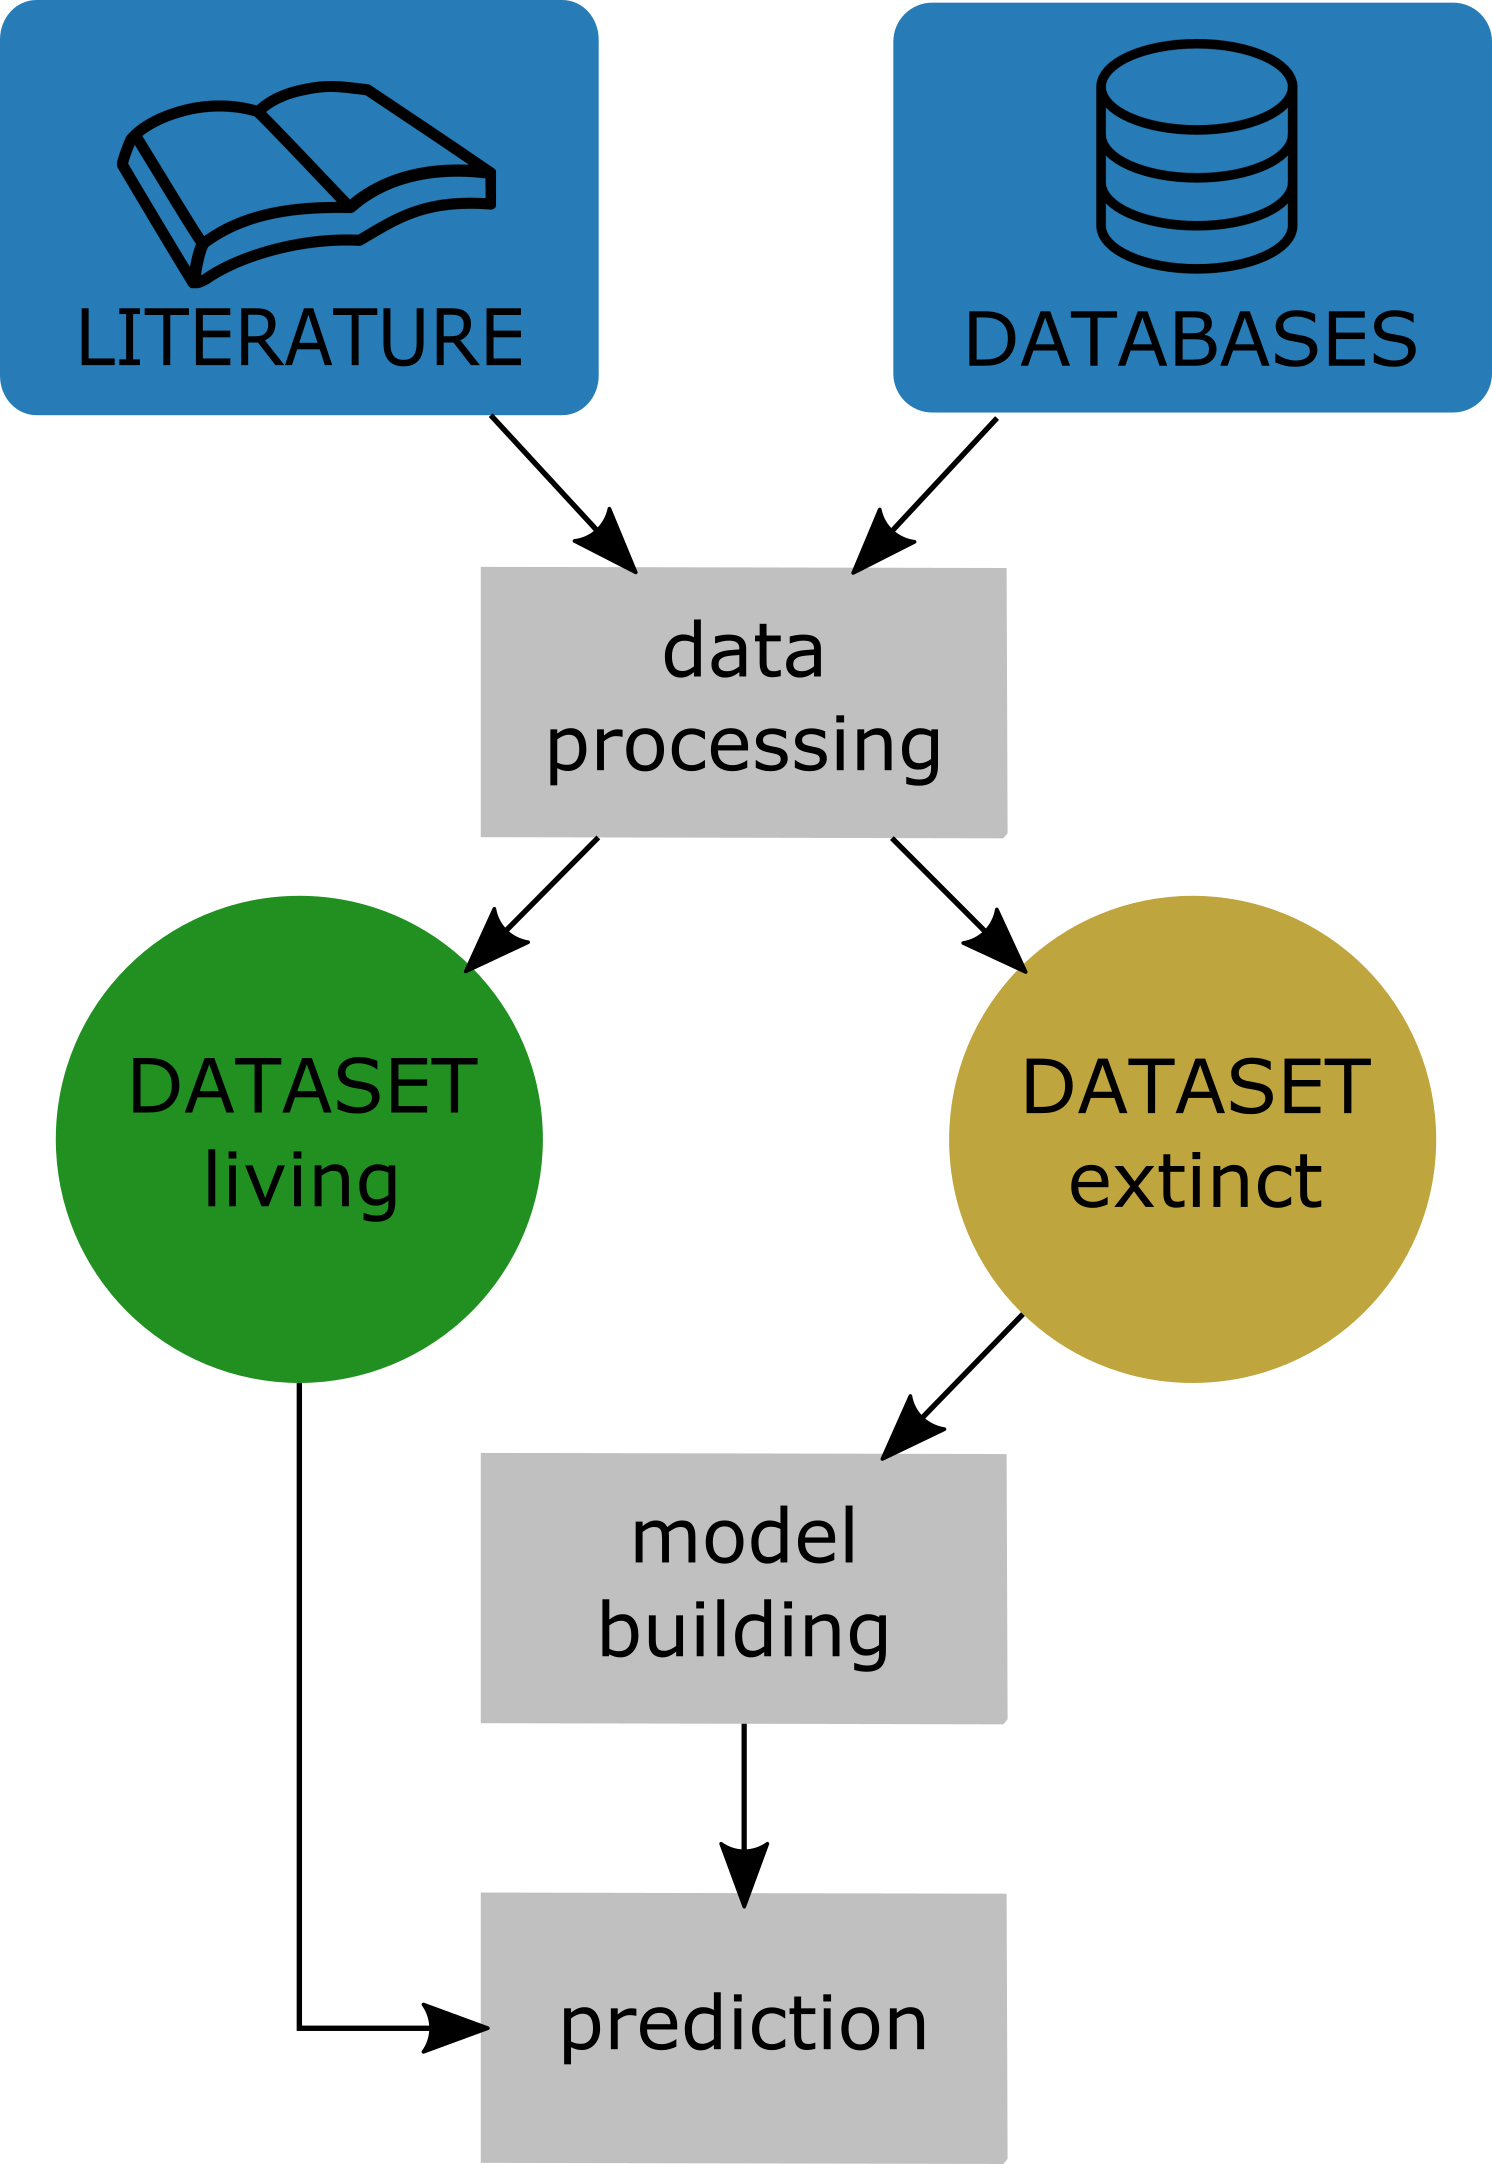
\includegraphics{model_framework.jpg}
\caption{}
\end{figure}

 Model framework for the study.
\href{https://doi.org/10.1111/ele.13080}{Tietje, M. and Rödel, M. O.
(2018), figure 1}.

We used generalised boosted modelling to analyse the impact of several
traits that are assumed to influence extinction risk on the
stratigraphic duration of amphibian species in the fossil record. We
used this fossil calibrated model to predict the extinction risk for
living species. We observed a high consensus between our predicted
species durations and the current IUCN Red List status of living
amphibian species. We also found that today's Data Deficient species are
mainly predicted to experience short durations, hinting at their likely
high threat status. Our study suggests that the fossil record can be a
suitable tool for the evaluation of current taxa specific Red Listing
status.

\begin{figure}
\centering
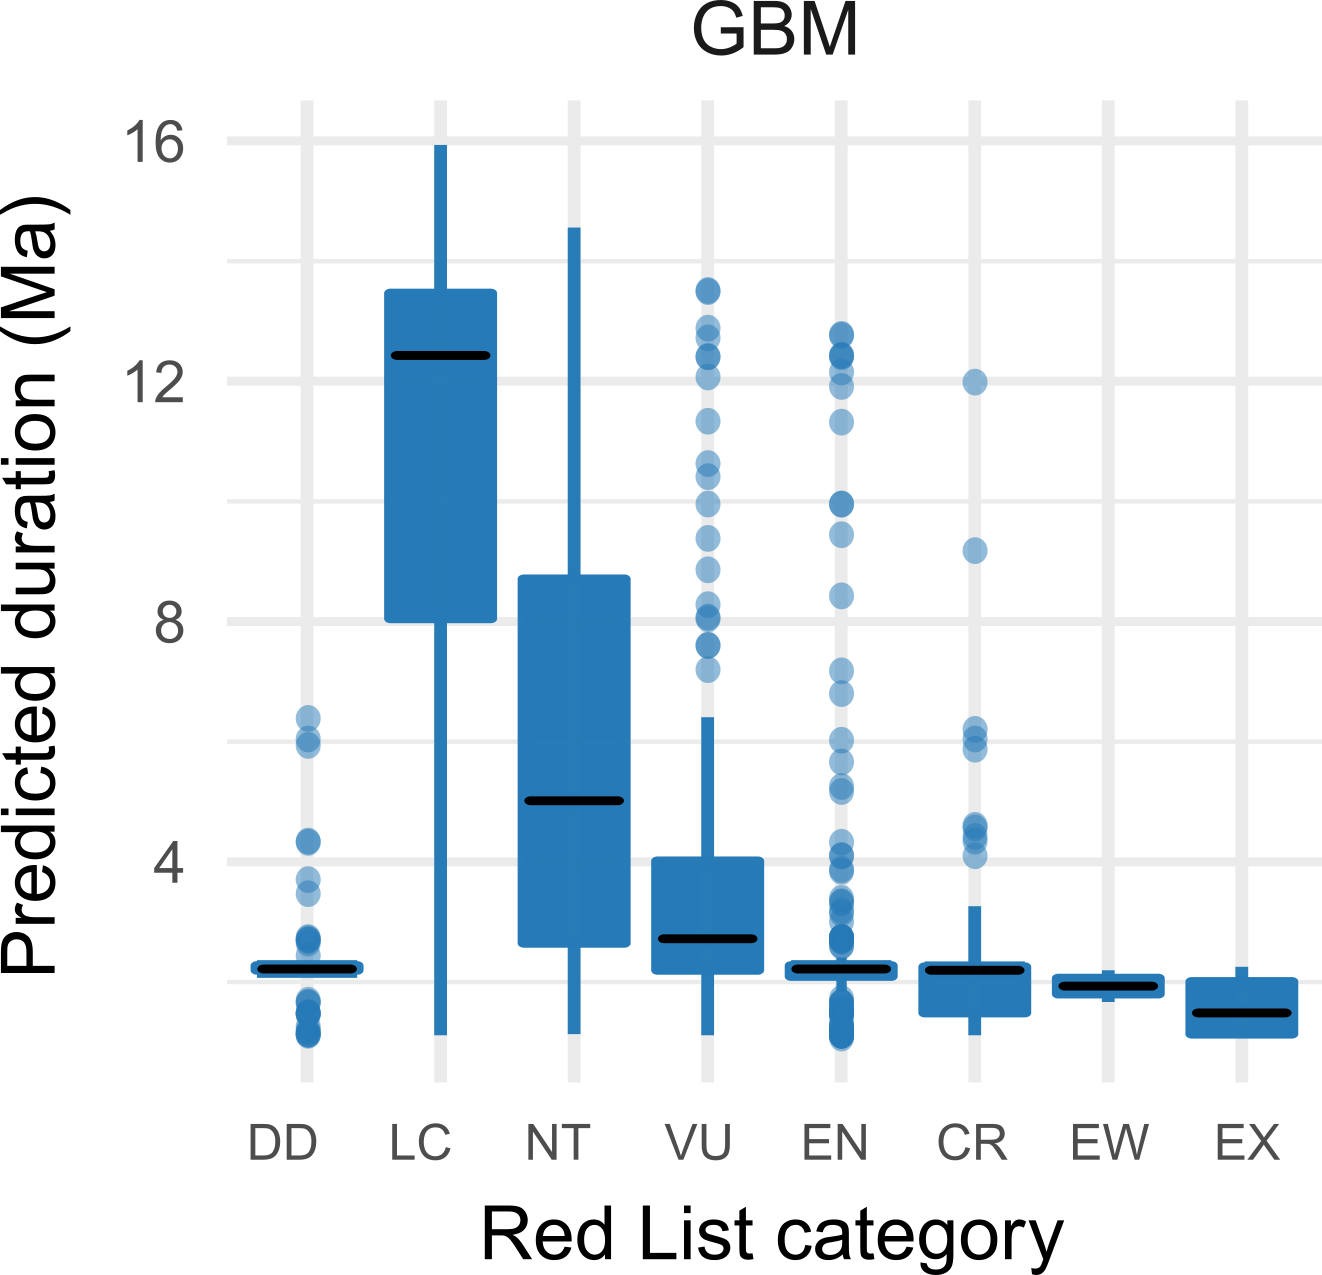
\includegraphics{figure3ELE.png}
\caption{}
\end{figure}

 Predicted durations in million years for living amphibian species,
based on the model fitted with paleontological data.
\href{https://doi.org/10.1111/ele.13080}{Tietje, M. and Rödel, M. O.
(2018), figure 3}.

\subsection{Literature}\label{literature-1}

\begin{enumerate}
\def\labelenumi{\arabic{enumi}.}
\tightlist
\item
  Baillie, J. E. M., Griffiths, J., Turvey, S. T., Loh, J. \& Collen, B.
  2010 Evolution Lost: Status and Trends of the World's Vertebrates.
  Zoological Society of London.
\item
  Sodhi, N. S., Bickford, D., Diesmos, A. C., Lee, T. M., Koh, L. P.,
  Brook, B. W., Sekercioglu, C. H. \& Bradshaw, C. J. A. 2008 Measuring
  the meltdown: drivers of global amphibian extinction and decline. PLoS
  One 3, e1636. (\url{doi:10.1371/journal.pone.0001636})
\item
  Harnik, P. G. 2011 Direct and indirect effects of biological factors
  on extinction risk in fossil bivalves. Proc. Natl. Acad. Sci. U. S. A.
  108, 13594--13599. (\url{doi:10.1073/pnas.1100572108})
\item
  Tietje, M. and Rödel, M. O. (2018), Evaluating the predicted
  extinction risk of living amphibian species with the fossil record.
  Ecology Letters.
  \href{https://doi.org/10.1111/ele.13080}{doi:10.1111/ele.13080}
\end{enumerate}


\end{document}
